% LaTeX and writing mathematics: the librarian's hour, framed, and the LaTeX
% and modularisation questions that come up once students start writing.
% Shared preamble for the write-on class slides.
%
% Every deck is designed to be projected and annotated live on a tablet:
% whatever takes time to draw is pre-drawn, and whatever the class produces is
% left blank. Compile a deck with `pdflatex main.tex` from its own directory,
% or run `uv run python build.py` from the repository root to build them all.
\documentclass[10pt]{article}

\usepackage[papersize={25.6cm,14.4cm}, margin=1.1cm, bottom=1.5cm,
            footskip=0.75cm]{geometry}
\usepackage[T1]{fontenc}
\usepackage[default]{sourcesanspro}
\usepackage{newtxsf}
\usepackage{tikz}
\usepackage{amsmath}
\usepackage{parskip}
\usepackage{fancyhdr}
\usetikzlibrary{arrows.meta, positioning, calc}

\setlength{\parindent}{0pt}

% Catppuccin Latte, the palette the course site uses in its light theme, so a
% deck on the projector looks like the pages the students read.
\definecolor{inkbg}{HTML}{EFF1F5}      % base
\definecolor{inksurface}{HTML}{E6E9EF} % mantle
\definecolor{inkfaint}{HTML}{CCD0DA}   % surface2, for rules and empty boxes
\definecolor{inktext}{HTML}{4C4F69}    % text
\definecolor{inkgrey}{HTML}{8C8FA1}    % overlay1, for anything secondary
\definecolor{inkblue}{HTML}{7287FD}    % lavender, the primary accent
\definecolor{inkteal}{HTML}{179299}    % teal
\definecolor{inkred}{HTML}{FE640B}     % peach, for whatever wants attention
\definecolor{inkmauve}{HTML}{8839EF}   % mauve

\pagecolor{inkbg}
\color{inktext}

% A box to write a short answer into. White against the tinted page, so it
% reads as somewhere to write rather than as part of the printed material.
\newcommand{\blank}[1][1.6]{%
  \tikz[baseline=(current bounding box.base)]{%
    \draw[inkfaint, line width=0.7pt, rounded corners=2pt, fill=white]
      (0,-0.18) rectangle (#1,0.62);}}

% A ruled area to work in. Faint dots keep handwriting level on a tablet.
\newcommand{\workspace}[2]{%
  \begin{tikzpicture}
    \draw[inkfaint, line width=0.7pt, rounded corners=3pt, fill=white]
      (0,0) rectangle (#1,#2);
    \foreach \gx in {0.5,1.0,...,#1}{%
      \foreach \gy in {0.5,1.0,...,#2}{%
        \fill[inkfaint] (\gx,\gy) circle (0.5pt);}}
  \end{tikzpicture}}

% A panel for material that is printed rather than written on.
\newcommand{\panel}[2]{%
  \begin{tikzpicture}
    \draw[inkfaint, line width=0.7pt, rounded corners=3pt, fill=inksurface]
      (0,0) rectangle (#1,#2);
  \end{tikzpicture}}

% A labelled card of printed material. #2 and #3 are widths in cm; the text
% column is the card less its padding, computed rather than guessed.
\newcommand{\cardbox}[4]{%
  \begin{tikzpicture}
    \node[draw=#1, line width=1pt, rounded corners=4pt, fill=white,
          minimum width=#2cm, minimum height=#3cm,
          text width=\dimexpr#2cm-0.9cm\relax,
          align=left, inner sep=0.45cm, text=inktext] {#4};
  \end{tikzpicture}}

% A card whose body is left blank for the class to fill in.
\newcommand{\cardblank}[4]{%
  \begin{tikzpicture}
    \node[draw=#1, line width=1pt, rounded corners=4pt, fill=white,
          minimum width=#2cm, minimum height=#3cm,
          text width=\dimexpr#2cm-0.9cm\relax,
          align=left, inner sep=0.45cm, text=inktext, anchor=north west]
      at (0,0) {#4};
  \end{tikzpicture}}

% Running header: the deck name on the left, the page's own step on the right.
% Each deck sets its name once with \deckname.
\newcommand{\deck}{}
\newcommand{\deckname}[1]{\renewcommand{\deck}{#1}}
\newcommand{\slidehead}[1]{%
  {\small\color{inkgrey}%
   \tikz[baseline=-0.5ex]{\fill[inkblue, rounded corners=1pt]
     (0,0) rectangle (0.22,0.22);}\;\deck
   \hfill \color{inkblue}\bfseries #1}\par
  {\color{inkblue}\rule{\linewidth}{1pt}}\par\vspace{0.35em}}

\pagestyle{fancy}
\fancyhf{}
\renewcommand{\headrulewidth}{0pt}
\fancyfoot[R]{\small\color{inkgrey}\thepage}

% Deck title pages, which carry no header and no page number.
\newcommand{\titleslide}[3]{%
  \thispagestyle{empty}%
  \begin{center}
    \vspace*{\fill}
    {\Huge\bfseries\color{inkblue} #1}\\[0.7em]
    {\LARGE\color{inkgrey} #2}\\[2.4em]
    #3
    \vspace*{\fill}
  \end{center}}

% One step of the plan on a title page.
\newcommand{\stepbox}[3]{%
  \node[draw=inkblue, line width=0.9pt, rounded corners=4pt, fill=white,
        minimum width=6cm, minimum height=1.7cm, align=center,
        text=inktext] (#1) at (#2,0) {#3};}

% Prompt to the room: a question the class answers, not something I read out.
\newcommand{\ask}[1]{%
  {\large\color{inkblue}\bfseries #1}\par\vspace{0.5em}}


\deckname{LaTeX and writing mathematics}

\begin{document}

\titleslide{LaTeX and writing mathematics}{Week 8. The paper starts here.}{%
    
\begin{tikzpicture}[font=\small]
      \stepbox{s0}{0.0}{\textbf{Frame}\\[0.25em] Research is 20\%.}
      \stepbox{s1}{6.9}{\textbf{Listen}\\[0.25em] The librarian's hour.}
      \stepbox{s2}{13.8}{\textbf{Write}\\[0.25em] The notes are yours.}
      \draw[-{Stealth[length=2.5mm]}, inkfaint, line width=1.2pt] (s0) -- (s1);
      \draw[-{Stealth[length=2.5mm]}, inkfaint, line width=1.2pt] (s1) -- (s2);
    \end{tikzpicture}}

\newpage
\slidehead{This hour is not a LaTeX lecture}

\vspace{0.9cm}

\begin{center}

\begin{tikzpicture}
  \node at (0,0) {\cardbox{inkblue}{10.4}{3.4}{%
    {\large\bfseries\color{inkblue} This hour}\\[0.5em]
    {\large The subject librarian, on finding\\ and judging sources.}}};
  \node at (12.6,0) {\cardbox{inkteal}{10.4}{3.4}{%
    {\large\bfseries\color{inkteal} Your own time}\\[0.5em]
    {\large The LaTeX notes, and the two\\ guides to writing mathematics.}}};
\end{tikzpicture}
\end{center}

\vspace{1.2cm}

\begin{center}
{\LARGE The two halves fit together. The notes teach you how to cite.\\
This hour is about \textbf{what is worth citing}.}
\end{center}

\newpage
\slidehead{Research is 20\% of the project mark}

\vspace{1.1cm}

{\LARGE
\textbf{\color{inkblue}State of the field.}\quad How does your library
compare with the tools that already exist?

\vspace{1.3em}

\textbf{\color{inkteal}References.}\quad Is everything that should be
cited actually cited, in the text, properly?}

\vspace{1.6cm}

\begin{center}
{\large\color{inkgrey} Four references the paper argues with beat twenty
in a bibliography the body never mentions.}
\end{center}

\newpage
\slidehead{Your state of the field, in one question}

\vspace{0.5cm}

\ask{Name three tools that already do something like what your library
will do. For each one, say what yours does differently.}

\vspace{0.3em}

\begin{center}
\workspace{22}{7.0}
\end{center}

\vspace{0.2cm}

{\small\color{inkgrey} `There is nothing else like it' is almost never
true, and it is the answer that scores worst.}

\newpage
\slidehead{This week's reading}

\vspace{1.1cm}

\begin{center}

\begin{tikzpicture}
  \node at (0,0) {\cardbox{inkblue}{10.4}{3.4}{%
    {\large\bfseries\color{inkblue} LaTeX}\\[0.5em]
    {\large Structure, mathematics, figures,\\ tables, bibliographies.}}};
  \node at (12.6,0) {\cardbox{inkteal}{10.4}{3.4}{%
    {\large\bfseries\color{inkteal} Modularisation of code}\\[0.5em]
    {\large One function doing one thing,\\ and importing a file.}}};
\end{tikzpicture}
\end{center}

\vspace{1.2cm}

\begin{center}
{\LARGE You read these \textbf{on your own}. The next five slides are the
parts that catch people.}
\end{center}

\newpage
\slidehead{Where is the title?}

\vspace{0.4cm}

\begin{minipage}[t]{0.48\linewidth}
\vspace{0pt}
\codebox{10.8}{\bs documentclass\{article\}\\[0.2em]
\bs title\{A library for ...\}\\
\bs author\{Our group\}\\
\bs date\{\bs today\}\\[0.3em]
\bs begin\{document\}\\
\idt Our library solves ...\\
\bs end\{document\}}
\end{minipage}
\hfill
\begin{minipage}[t]{0.48\linewidth}
\vspace{0pt}
\ask{This compiles without an error, and the title is nowhere on the
page. Why?}

\workspace{11.0}{6.0}
\end{minipage}

\vspace{0.2cm}

{\small\color{inkgrey} The preamble says what the title is.
\texttt{\bs maketitle} is what puts it on the page.}

\newpage
\slidehead{Why is my citation a question mark?}

\vspace{1.0cm}

\begin{center}

\begin{tikzpicture}
  \foreach \lbl/\x/\n in {pdflatex/0/a, bibtex/5.6/b, pdflatex/11.2/c,
                          pdflatex/16.8/d}{%
    \node[draw=inkblue, line width=1pt, rounded corners=4pt, fill=white,
          minimum width=4.4cm, minimum height=1.8cm, font=\large\ttfamily,
          text=inkblue] (\n) at (\x,0) {\lbl};}
  \foreach \p/\q in {a/b, b/c, c/d}{%
    \draw[-{Stealth[length=2.5mm]}, inkfaint, line width=1.3pt] (\p) -- (\q);}
\end{tikzpicture}
\end{center}

\vspace{1.3cm}

\ask{You ran \texttt{pdflatex} once and the paper says \texttt{[?]}.
Which of these four have you not done?}

\vspace{0.2em}

\begin{center}
\workspace{22}{3.4}
\end{center}

\vspace{0.2cm}

{\small\color{inkgrey} Overleaf does all four for you. A local build does
not. Cross references need the second \texttt{pdflatex} too.}

\newpage
\slidehead{Two habits to drop}

\vspace{0.8cm}

\begin{center}
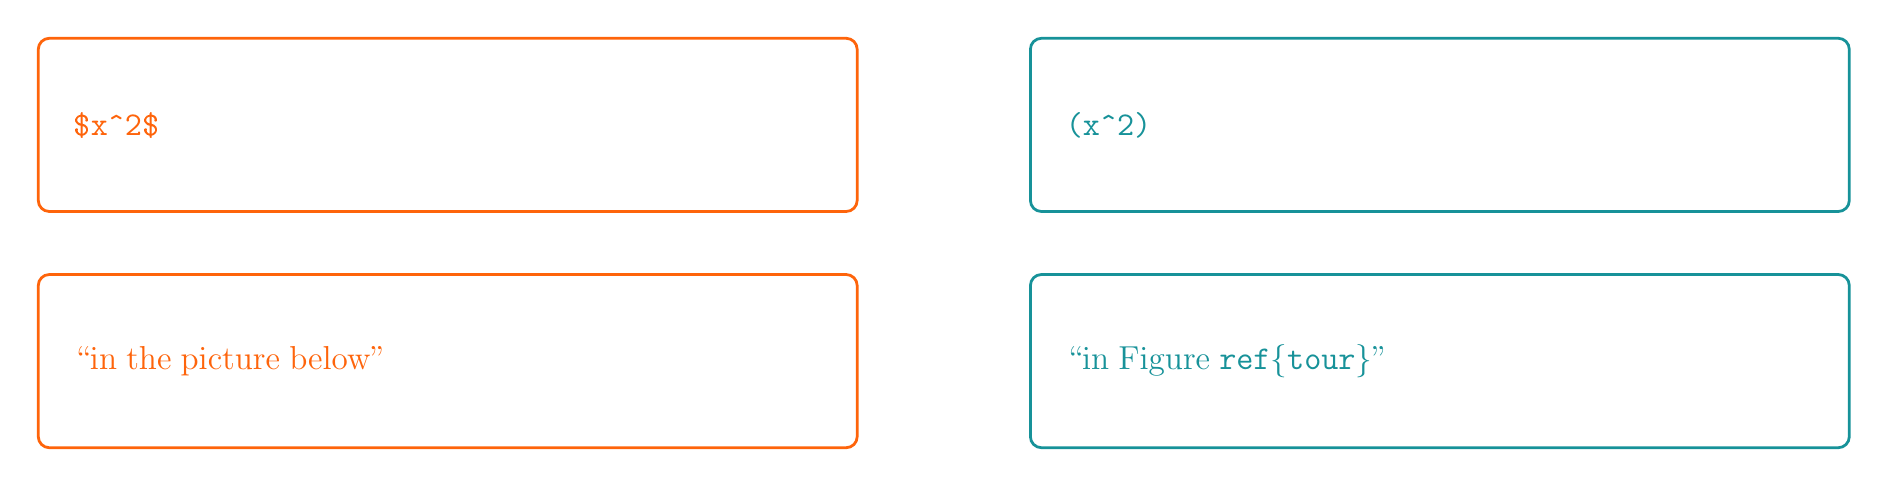
\begin{tikzpicture}
  \node at (0,0) {\cardbox{inkred}{10.4}{2.2}{%
    {\large\ttfamily\color{inkred} \$x\textasciicircum 2\$}}};
  \node at (12.6,0) {\cardbox{inkteal}{10.4}{2.2}{%
    {\large\ttfamily\color{inkteal} \bs(x\textasciicircum 2\bs)}}};
  \node at (0,-3.0) {\cardbox{inkred}{10.4}{2.2}{%
    {\large\color{inkred} ``in the picture below''}}};
  \node at (12.6,-3.0) {\cardbox{inkteal}{10.4}{2.2}{%
    {\large\color{inkteal} ``in Figure~\texttt{\bs ref\{tour\}}''}}};
\end{tikzpicture}
\end{center}

\vspace{1.0cm}

\ask{The second one is not a matter of taste. What goes wrong?}

\vspace{0.3cm}

{\small\color{inkgrey} A figure is a float. LaTeX puts it where it fits,
which may not be below anything.}

\newpage
\slidehead{Name this function without using `and'}

\vspace{0.5cm}

\begin{center}
\codebox{20.4}{def add\_tip\_and\_get\_bill\_share(total, tip\_proportion,
number\_of\_payers):\\
\idt tip\_amount = tip\_proportion * total\\
\idt return (total + tip\_amount) / number\_of\_payers}
\end{center}

\vspace{0.7cm}

\ask{You cannot. So how many functions is this, and what are they called?}

\vspace{0.3em}

\begin{center}
\workspace{22}{4.0}
\end{center}

\vspace{0.2cm}

{\small\color{inkgrey} Small enough to test on its own, and nameable
without `and'. A better rule than counting lines.}

\newpage
\slidehead{Why did importing it draw a plot?}

\vspace{0.4cm}

\begin{minipage}[t]{0.46\linewidth}
\vspace{0pt}
\codebox{10.4}{\# tsp.py\\[0.2em]
def get\_cost(tour, matrix):\\
\idt ...\\[0.4em]
\wrong{tour = get\_tour(25)}\\
\wrong{plot\_tour(x, y, tour)}}
\end{minipage}
\hfill
\begin{minipage}[t]{0.50\linewidth}
\vspace{0pt}
\ask{Another group types \texttt{import tsp} and a figure appears. What
happened?}

\workspace{11.4}{6.0}
\end{minipage}

\vspace{0.2cm}

{\small\color{inkgrey} Importing a file runs everything at its top level.
Your library holds functions. The code that uses them lives elsewhere, or
under \texttt{if \_\_name\_\_ == "\_\_main\_\_":}.}

\newpage
\slidehead{Before you leave}

\vspace{0.8cm}

\begin{center}
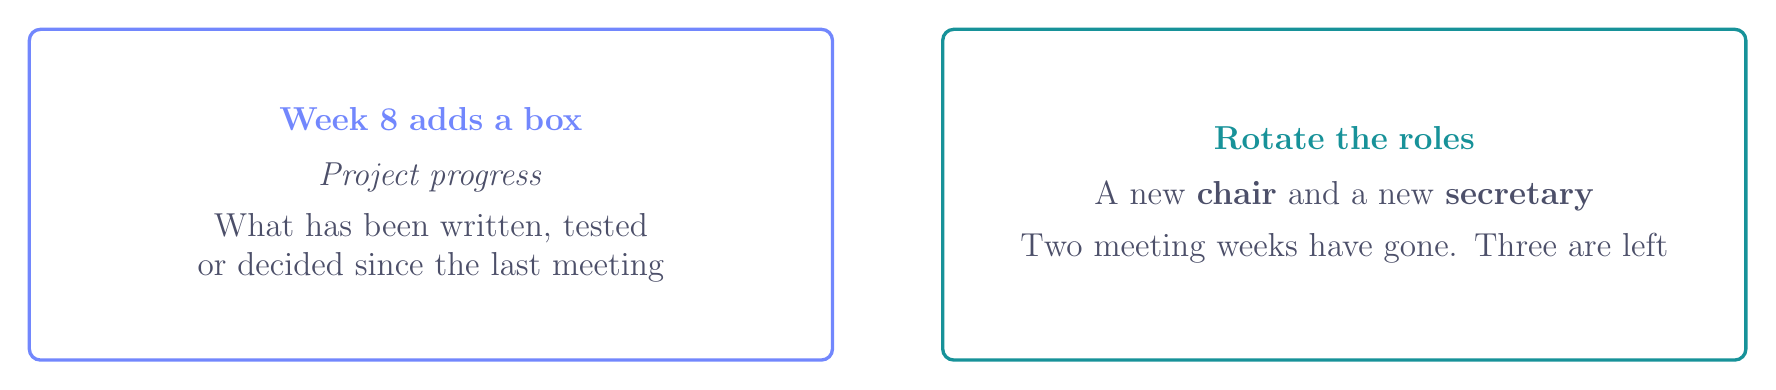
\begin{tikzpicture}
  \node[draw=inkblue, line width=1.2pt, rounded corners=4pt, fill=white,
        minimum width=10.2cm, minimum height=4.2cm, text width=9.2cm,
        align=center, inner sep=0.4cm, text=inktext, font=\large] at (0,0) {%
    \textbf{\color{inkblue} Week 8 adds a box}\\[0.5em]
    \emph{Project progress}\\[0.4em]
    What has been written, tested or decided since the last meeting};
  \node[draw=inkteal, line width=1.2pt, rounded corners=4pt, fill=white,
        minimum width=10.2cm, minimum height=4.2cm, text width=9.2cm,
        align=center, inner sep=0.4cm, text=inktext, font=\large]
    at (11.6,0) {%
    \textbf{\color{inkteal} Rotate the roles}\\[0.5em]
    A new \textbf{chair} and a new \textbf{secretary}\\[0.4em]
    Two meeting weeks have gone. Three are left};
\end{tikzpicture}
\end{center}

\vspace{0.9cm}

\begin{center}

\begin{tikzpicture}
  \node[draw=inkred, line width=1.4pt, rounded corners=4pt, fill=white,
        minimum width=21.8cm, minimum height=2.2cm, text width=20.6cm,
        align=center, inner sep=0.35cm, text=inktext, font=\large] {%
    \textbf{\color{inkred} Meet this week. Bring the Week 8 minutes to the
    next session.}\quad The third of the five that \(I\) is counted from.};
\end{tikzpicture}
\end{center}

\end{document}
